Distributed systems typically consist of two or more components that communicate \emph{asynchronously} by sending and receiving messages through a network layer. When a component receives a message, it responds by executing a predefined \emph{message handler}. This handler consists of a sequence of program statements that might update the internal state of the component, send a message to another component in the system, or even create an entirely new component.

As an example of a distributed system, Figure~\ref{fig:azurestore} shows the top-level components of Azure Storage vNext, a distributed extent management system for Windows Azure that is used in production inside Microsoft. Azure Storage vNext consists of multiple extent managers, extent nodes and a remote procedure call (RPC) communication engine. Each extent manager is responsible for managing a subset of the extent nodes. Each extent node is responsible for storing its corresponding extent in a local storage. Finally, the RPC engine is responsible for sending messages across the network, and enqueuing any received messages in the inbox queue of the corresponding node. This system is described in more details in Section~\ref{sec:cases:azurestore}.

\subsection{Testing distributed systems}
\label{sec:overview:bugs}

In a distributed system, message handlers can interleave in arbitrary order, because of the asynchronous nature of message-based communication. To complicate matters further, unexpected failures are the norm in production: nodes in a cluster might fail at any moment, and thus programmers have to implement sophisticated mechanisms that can deal with these failures and recover the state of the system. Moreover, with multicore machines having become a commodity, individual components of a distributed system are commonly implemented using multithreaded code, which adds another source of nondeterminism.

\begin{figure}[t]
\centering
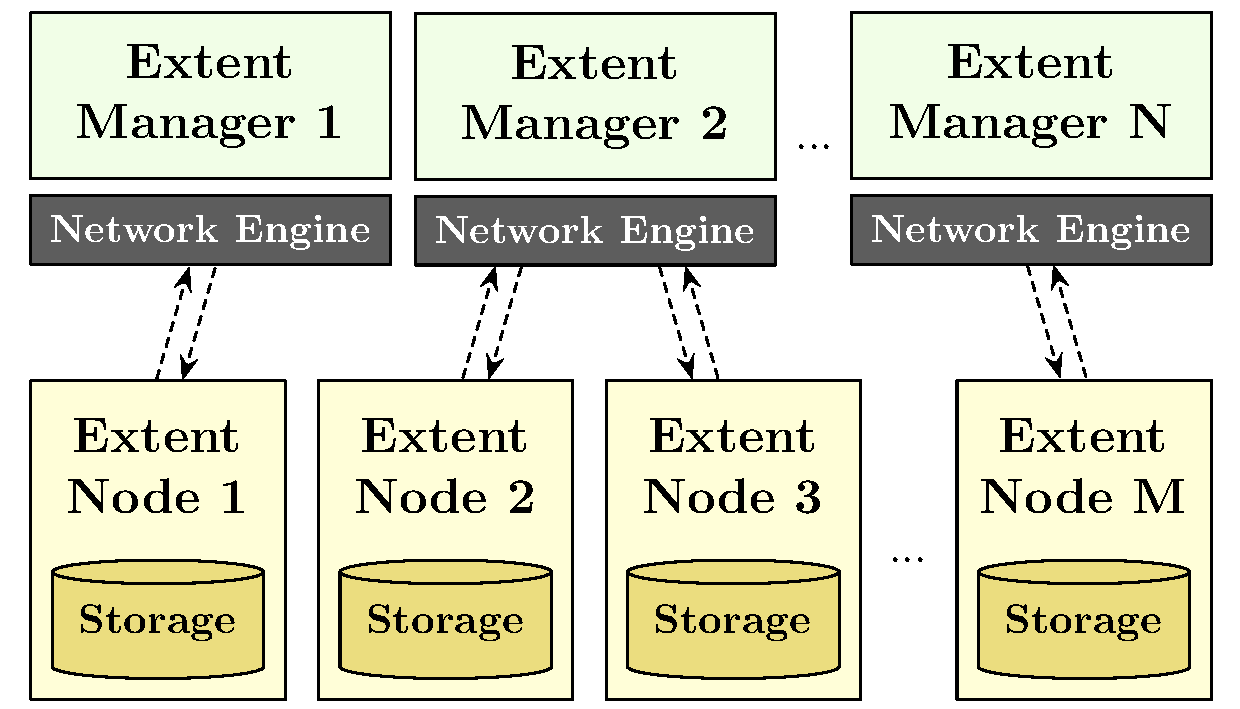
\includegraphics[width=\linewidth]{img/azurestore}
\caption{Top-level components of a distributed extent management system for Windows Azure.}
\label{fig:azurestore}
\end{figure}

All these sources of nondeterminism (as well as nondeterminism due to timeouts, message losses and client requests) can easily create \emph{heisenbugs}~\cite{musuvathi2008finding}, which are corner-case bugs that are difficult to detect, diagnose and fix, without using advanced \emph{asynchrony-aware} testing techniques.
%
The ideal testing tool should be able to work on unmodified systems, capture and control all possible sources of nondeterminism, systematically inject faults in the right places, and explore all feasible execution paths. However, this is easier said than done when testing production systems.

\subsection{Bugs in distributed systems}
\label{sec:overview:bugs}

There are two types of properties that developers of distributed systems are mostly interested in testing: \emph{safety} and \emph{liveness} properties. A safety property holds if it is \emph{always} satisfied, i.e. holds invariantly in every program state during execution. Likewise, a liveness property holds if it becomes \emph{eventually} satisfied, i.e. it will hold at some program state during execution. A safety or liveness property violation means that there is a bug that should be fixed.

Examples ...

How cheng was testing his code before and how after -- high level, pretty picture

